We would like to to observe and study how validity cores evolves over unrolling the transition relation. It is interesting to see how quickly validity cores from a bounded proof converges to an actual minimal IVC.

Note that the purpose of our experiments on BVCs is mostly to point out some research directions. Further studies may even can make use of BVCs in verification problems. A lot of time a valid property is hard or not inductive for the model checker to prove. In such cases, looking at the history of BVC runs may give us some confidence about the correctness of the property. The experimental results show that when we reach one of the actual MIVCs, BVC runs result in the same cores over and over. That is to say, when the BVC runs come to stable cores, it may imply we might have already seen all the reachable states, and implicitly known they are safe. Although this hypothesis may not be true and the reverse does not necessarily hold, it may be worth further investigations.

\subsection{Experimental Setup}
  We perform our experiments on the same benchmark suite with 660 models introduced in Section \ref{sec:expsetup}. The experiment is conducted with a maximum depth of 10 and one hour timeout; i.e. for each model, if unrolling to depth 10 takes more than one hour, the \bvcalg\ algorithm will terminate. We capture $\bvc _{k}$ for $ 0 \leq k \le 10$, then compare each \bvc\ of depth $k$ to see how they change during unrolling. Then, the final bounded validity cores obtained from at the maximum\footnote{Maximum depth in this experiment is 10. For most of the models, it is possible to reach this depth in less than an hour.}
  reachable depth in one hour, denoted by $\bvc _{max}$ , are considered as our final cores. These cores are compared with all the MIVCs gathered in Section \ref{subsec:res} to see if they match up with any of the actual minimal IVCs.

Research questions we would like to answer in this study are as follows:
\begin{itemize}
  \item \textbf{RQ1:} How many of the final \bvc s match one of the \mivc s?
  %How many of the final BVCs do match up with one of the MIVCs? For how many of the models does the algorithm time out?
  \item \textbf{RQ2:} How do \bvc s evolve as the analysis depth changes?
  %At what rate does size of the BVCs change? Does the size of the cores increase with the depth?
  \item \textbf{RQ3:} Is there a relationship between size and structure of models and the size of \bvc s and the rate at which they converge with a \mivc?
  %How close is $\bvc _{max}$ to an actual MIVC? Is there any relationship with the size of the models and convergence of the BVCs?
\end{itemize}

\vspace{0.1in}
\subsubsection{RQ1}
The result of the experiments show that $\bvc _{max}$ is the same as one of the MIVCs for 474 models out of 660. For 27 of the models, $\bvc _{max}$ was not subset of any MIVCs (had additional elements, also none of the MIVCs was a subset of the $\bvc _{max}$)\footnote{We will explain the reason in \textbf{RQ2}}. However, $\bvc _{max}$ was a subset of one of the MIVCs in 159 of the models.

We performed the experiments with \texttt{Z3} and \texttt{Yices} solvers. UNSAT core generation in \texttt{Z3} is faster, and \texttt{JKind} has special hack to get UNSAT cores from \texttt{Yices} because it does not have a support for it. Using \texttt{Z3}, 12 of the models did not reach depth 10 in one hour. With \texttt{Yices}, 18 of the models timed out. An interesting fact is that we had models that did not reach $\bvc _{10}$, but their $\bvc _{max}$ was the same as one of the MIVCs. For example, one of the models containing 571 design elements only reached to $\bvc _{2}$, but $\bvc _{2}$ was the same as one of the MIVCs.
The BVC size for that model at different depths is as follows:\footnote{This particular model is named ``steam\_boiler\_no\_arr1.lus'' in our benchmarks. You can see the results and model in our experimental directories \cite{expr}.}

$|\bvc _{0}| = 6$, $|\bvc _{1}| = 11$, $|\bvc _{2}| = 128$

There are interesting case studies where from the initial depth, the BVC was the same as one of the MIVCs. For example, in our benchmark we have a model with 27 design element\footnote{File ``car\_all\_e8\_856\_e2\_585.lus'' in our benchmark directory.}, for which $|\bvc _{i}| = 5$, $i \leq 0 \le 10$, and $\bvc _{0}$ is the same as its only one MIVC.

\vspace{0.1in}
\subsubsection{RQ2}
Our experimental results show that among 474 models for which $\bvc _{max}$ is the same as one of the MIVCs, the size of the BVCs were (nonstrictly) increasing 99.9\% of the time:
      $$ 0 \leq i \le max, |\bvc _{i}| \leq |\bvc _{i+1}|$$
      In other words, for only 12 of these models, the above relation did not hold.
      It is expected that bounded cores in each unrolling step (nonstrictly) increases as in each step more states are being reached and the cores required for the proof of the property is more likely to expand.
      We run the experiments over those 12 models with different solvers (once with \texttt{Z3} and once with \texttt{Yices}). In both runs, these models, mostly, behave the same (except 3 of them; see Table \ref{tab:bvc-abnormal}).

      It is interesting to see why those 12 models show different behavior. By looking at different case studies, we have found three main reasons that explain this anomaly.  The first explanation is that when a model has several distinct MIVCs, the bounded core could change during unrolling. However, we examined these models and there are ones with a single MIVC that behaved abnormally. Another explanation for such models is that MIVCs obtained from \aivcalg ~contained timeout loops; therefore, we do not have the exact minimal IVCs for those cases (for example model\#6 in Table \ref{tab:bvc-abnormal}).

       The result of BVC runs for these models (on \texttt{Yices}) is shown in Table \ref{tab:bvc-abnormal}.


      % (a) shows a picture containing all the models. Figure  \ref{fig:bvc-growth} (b) is the enlarged version for some of the smaller models, and Figure  \ref{fig:bvc-growth} (c) magnifies the parts for larger models.



\begin{table}
  \caption{BVC runs for the models with non-increasing behavior where $\bvc _{max}$ is the same as one of the MIVCs.}

  \centering
  \begin{tabularx}{\linewidth}{ |c||c|c|c|c|c|c|c|c|c|c||L|L|}
    \hline
    $|\bvc _{i}|$ ~/~ $i=$ & 0 & 1 & 2 & 3 & 4 & 5 & 6 & 7 & 8 & 9 & \small{model size} & \small{\#of MIVCs} \\[0.5ex]
    \hline\hline

    model\#1& 2 & 9 & 34 & 36& 28 & 28 & 28 & 28 & 28 & 28 & 70&1 \\[0.5ex]
    model\#2& 5 & 15 & 11& 11& 11 & 11 & 11 & 11 & 11 & 11 & 123 &1\\[0.5ex]
    model\#3& 8 & 9& 13& 33& 28& 40& 38& 41& 41& 41&57 &7 \\[0.5ex]
    model\#4& 2& 5& 8& 10& 12& 10& 10& 10& 10& 10 &64 &9\\[0.5ex]
    \small{model\#5 (\texttt{Yices})}&9& 24 & 84& 84& 82& 82& 82& 82& 82& 82&96 &1\\[0.5ex]
    \small{model\#5 (\texttt{Z3})}& 9& 24& 82& 82& 82& 82& 82& 82& 82& 82&96 &1\\[0.5ex]
    model\#6& 5& 6& 5& 7& 5& 7& 5& 7& 5& 7& 7 &1\\[0.5ex]
    model\#7& 5& 6& 6& 5& 5& 6& 6& 5& 5& 6&6 &1\\[0.5ex]
    \small{model\#8 (\texttt{Yices})}& 9& 12& 14& 28& 37& 36& 36& 36& 36& 36&103&1 \\[0.5ex]
    \small{model\#8 (\texttt{Z3})}&9& 12& 14& 28& 37& 37& 37& 37& 37& 37& 103&1\\[0.5ex]
    \small{model\#9 (\texttt{Yices})}& 2& 6& 10& 4& 4& 4& 4& 4& 4& 4 &64&1 \\[0.5ex]
    \small{model\#9 (\texttt{Z3})}& 2& 4& 4& 4& 4& 4& 4& 4& 4& 4 &64&1\\[0.5ex]
    model\#10& 2& 6& 8& 11& 7& 7& 7& 7& 7& 7 &64&1\\[0.5ex]
    model\#11& 4& 13& 32& 47& 61& 54& 54& 54& 54& 54 &103&8 \\[0.5ex]
 \small{model\#12 (\texttt{Yices})}& 8& 8& 21& 29& 39& 38& 38& 40& 41& 41&57&6\\[0.5ex]
  \small{model\#12 (\texttt{Z3})}& 8& 17& 21& 29& 32& 38& 38& 32& 32& 32&57&6 \\[0.5ex]
    \hline
  \end{tabularx} \\
%{Actual model names in Table \ref{tab:bvc-abnormal}\\model\#1: fast\_1\_e8\_751.lus \\model\#2: microwave05.lus\\mode\#3: DRAGON\_12.lus\\model\#4: Display\_Control-Gaurantee0
%  \\model\#5:fast\_2\_e8\_976.lus
%  \\model\#6: twisted\_counters.lus
%  \\model\#7: two\_counters.lus
%  \\model\#8: cruise\_controller\_04.lus
%  \\model\#9: Display\_Control-Gaurantee2.lus
%  \\model\#10: Display\_Control-Gaurantee1.lus
%  \\model\#11: cruise\_controller\_24.lus
%  \\model\#12: DRAGON\_13.lus}
\vspace{0.07in}
{\small{Actual model names in the benchmark, respectively: fast\_1\_e8\_751.lus, microwave05.lus, DRAGON\_12.lus, Display\_Control-Gaurantee0, fast\_2\_e8\_976.lus, twisted\_counters.lus, two\_counters.lus, cruise\_controller\_04.lus, Display\_Control-Gaurantee2.lus, Display\_Control-Gaurantee1.lus, cruise\_controller\_24.lus, DRAGON\_13.lus}}
  \label{tab:bvc-abnormal}
\end{table}

The third reason why the size of BVCs is not always increasing is more interesting, which also explains why in some cases $\bvc _{max}$ is not the subset of any of the MIVCs. This only has to do with the depth of bounded model checking. In some problems, when we are at the earlier steps of unrolling transition relation (i.e. lower depths), the property can be satisfied in different ways. In other words, a property may have multiple \bvc s at depth $k$, but as we advance towards the deeper bounds leading to a proof, the validity cores converges to a smaller subset.
For clarification, let us take a look at one of the models small enough to discuss. This model is named \emph{ex3\_e8\_381\_e7\_224} in our benchmarks (Figure \ref{fig:expl}). It only has one MIVC ({\small{\texttt{\{V19\_late, V64\_incr, V63\_diff, V65\_PC, OK\}}}}), and \jkind is able to prove its property in less than a second. In addition, for this model, there is no timeout issue in the inner loops of \aivcalg\ algorithm. Using \texttt{Yices} in our experiments, $\bvc _{max}$ is not the subset of the only MIVC that this model has. However if we had just increased the depth by 1, from $\bvc _{10}$ on, the BVC would have become the same as the MIVC. For this model, up to depth 10, we have two ways of satisfying the property (we have two bounded validity cores {\small{\texttt{\{V19\_late, V64\_incr, V63\_diff, V65\_PC, OK\}}}} and {\small{\texttt{\{V20\_early, V64\_incr, V63\_diff, V65\_PC, OK\}}}}), but after depth 10, the property is satisfied with only one validity core ({\small{\texttt{\{V19\_late, V64\_incr, V63\_diff, V65\_PC, OK\}}}}). Figure \ref{fig:explout} shows the output of the \jkind BVC engine over this model up to depth 15.

 \begin{figure}
 \centering
  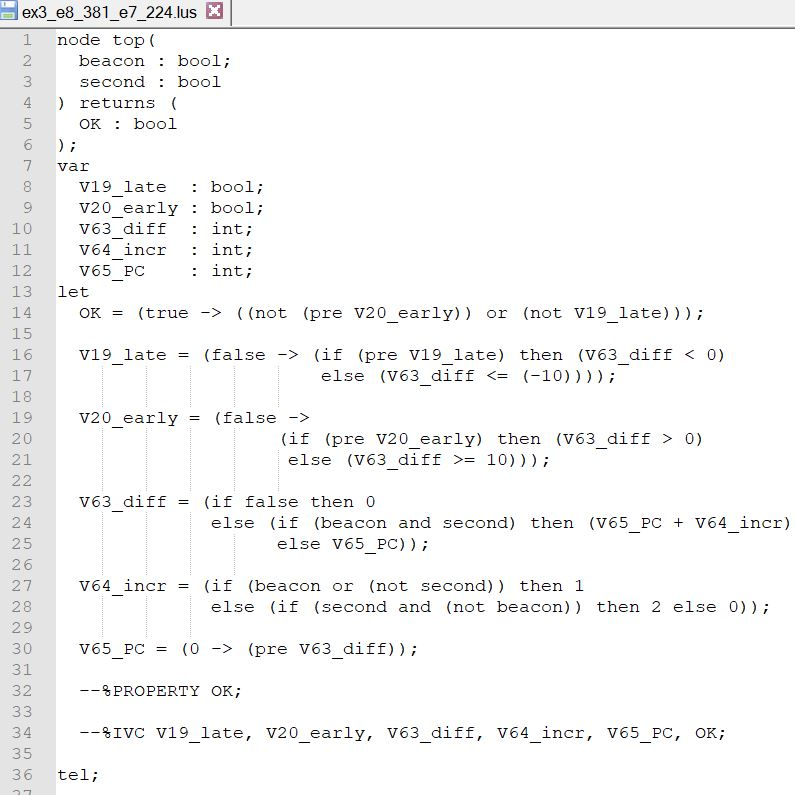
\includegraphics[width=\columnwidth]{figs/expl.jpg}
  %\vspace{-0.1in}
  \caption{Model ex3\_e8\_381\_e7\_224 as a case study}
  \vspace{0.1in}
  \label{fig:expl}
\end{figure}

\begin{figure}
 \centering
  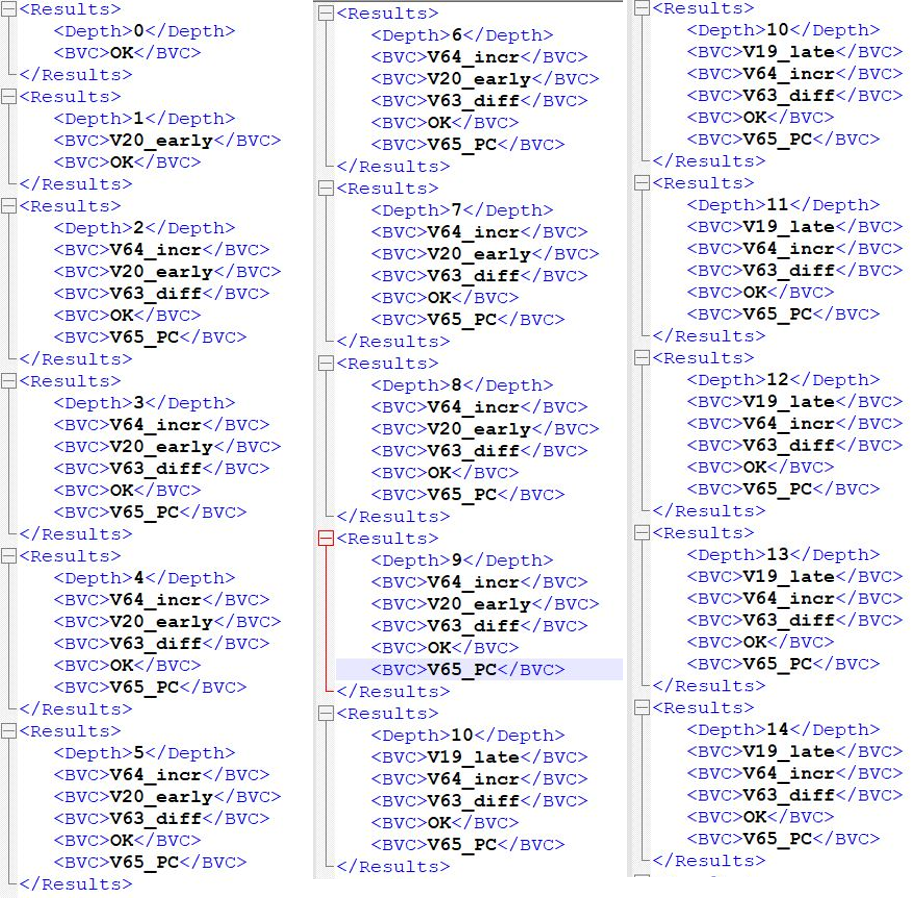
\includegraphics[width=\columnwidth]{figs/explout.png}
  %\vspace{-0.1in}
  \caption{BVC runs for model ex3\_e8\_381\_e7\_224}
  \vspace{0.1in}
  \label{fig:explout}
\end{figure}


\vspace{0.1in}
\subsubsection{RQ3}
In order to show how quickly BVCs change and converge to an actual MIVC, we chose $\bvc _{0}$, $\bvc _{3}$, and $\bvc _{max}$  runs and plot the size of the cores. Mostly for models with less than 200 design elements, size of BVCs did not change much from depth 3 to 9. For the larger models there is some difference between the size of $\bvc _{3}$ and $\bvc _{max}$ (Figure \ref{fig:bvc-growth}).


 \begin{figure}
 \centering
  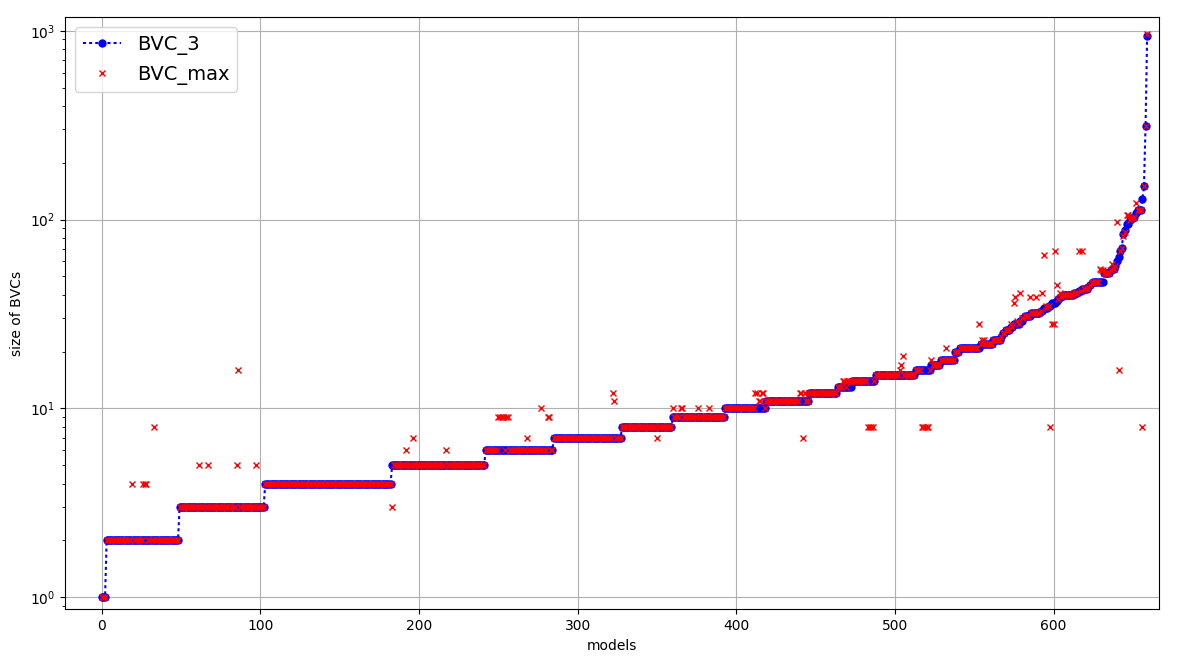
\includegraphics[width=.85\columnwidth]{figs/bvcmax.png}
  %\vspace{-0.1in}
  \caption{Size of BVCs at depth 3 and max}
  \vspace{0.1in}
  \label{fig:bvc-growth}
\end{figure}


We calculated the difference of $\bvc _{max}$ of each model with its MIVCs. Part of the results is described in \textbf{RQ1}. If $\bvc _{max}$  is the subset of one of the MIVCs, we calculated the difference between those two, and if not, $\bvc _{max}$  is compared with one of the MIVCs of the model, selected randomly.  Note that it is possible for $\bvc _{max}$ to be a subset of more than one of the MIVCs. In our calculation, we randomly selected the first MIVC containing $\bvc _{max}$.
%Figure \ref{fig:dif-bvc} visualizes the results.
Figure \ref{fig:bvc-size} shows the size of the models versus the size differences of MIVCs and BVCs
%line from Figure \ref{fig:dif-bvc}
in logarithmic scale.

% \begin{figure}
% \centering
%  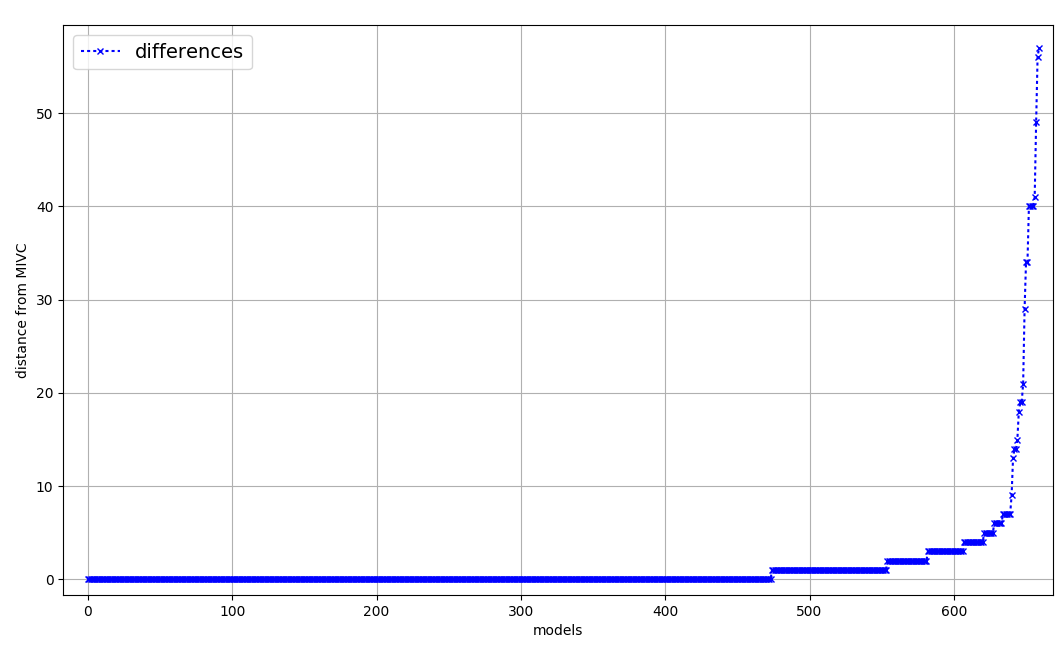
\includegraphics[width=\columnwidth]{figs/bvc_dif_yices.png}
%  %\vspace{-0.1in}
%  \caption{Difference between $\bvc _{max}$ and MIVCs}
%  \vspace{0.1in}
%  \label{fig:dif-bvc}
%\end{figure}

 \begin{figure*}
 \centering
  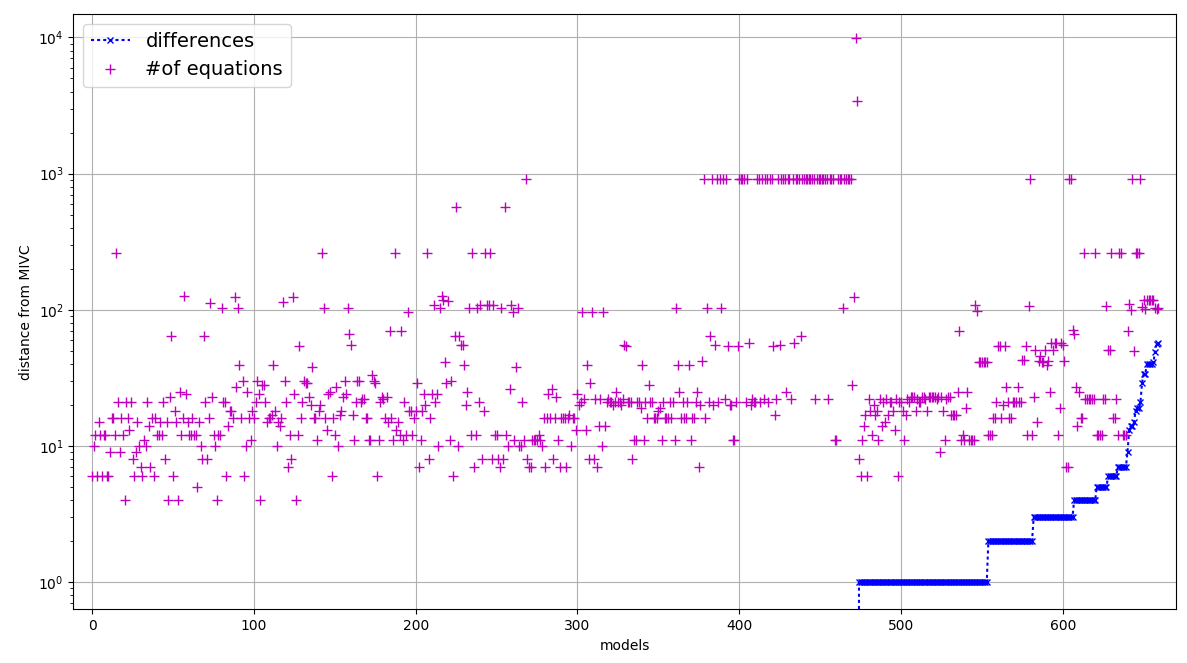
\includegraphics[width=\columnwidth]{figs/bvc_modelsize_yices.png}
  %\vspace{-0.1in}
  \caption{Difference between $\bvc _{max}$ and MIVCs vs the model size}
  \vspace{0.1in}
  \label{fig:bvc-size}
\end{figure*}

\vspace{0.1in}
\subsubsection{Discussion}
Experimental results show that in many cases, bounded validity cores can be as accurate as actual minimal IVCs. The abnormal behavior in some cases showed that we cannot make a strong claim about the relationships between BVCs and IVCs. One observation is that at deeper bounds, we can have more accurate bounded validity cores. The more accurate bounded cores are, the more useful information we have to evaluate completeness and adequacy of proofs. It may be possible to make use of other techniques to evaluate the accuracy of the bounded cores. For example, in case of non-increasing BVCs, we may build different abstractions for the model using different BVCs, and try to prove the property over abstracted models. If property fails over one abstraction, we can easily rule out the bounded core used for that abstraction. 